\textbf{Technologies}

\begin{figure}[h]
  \centering
  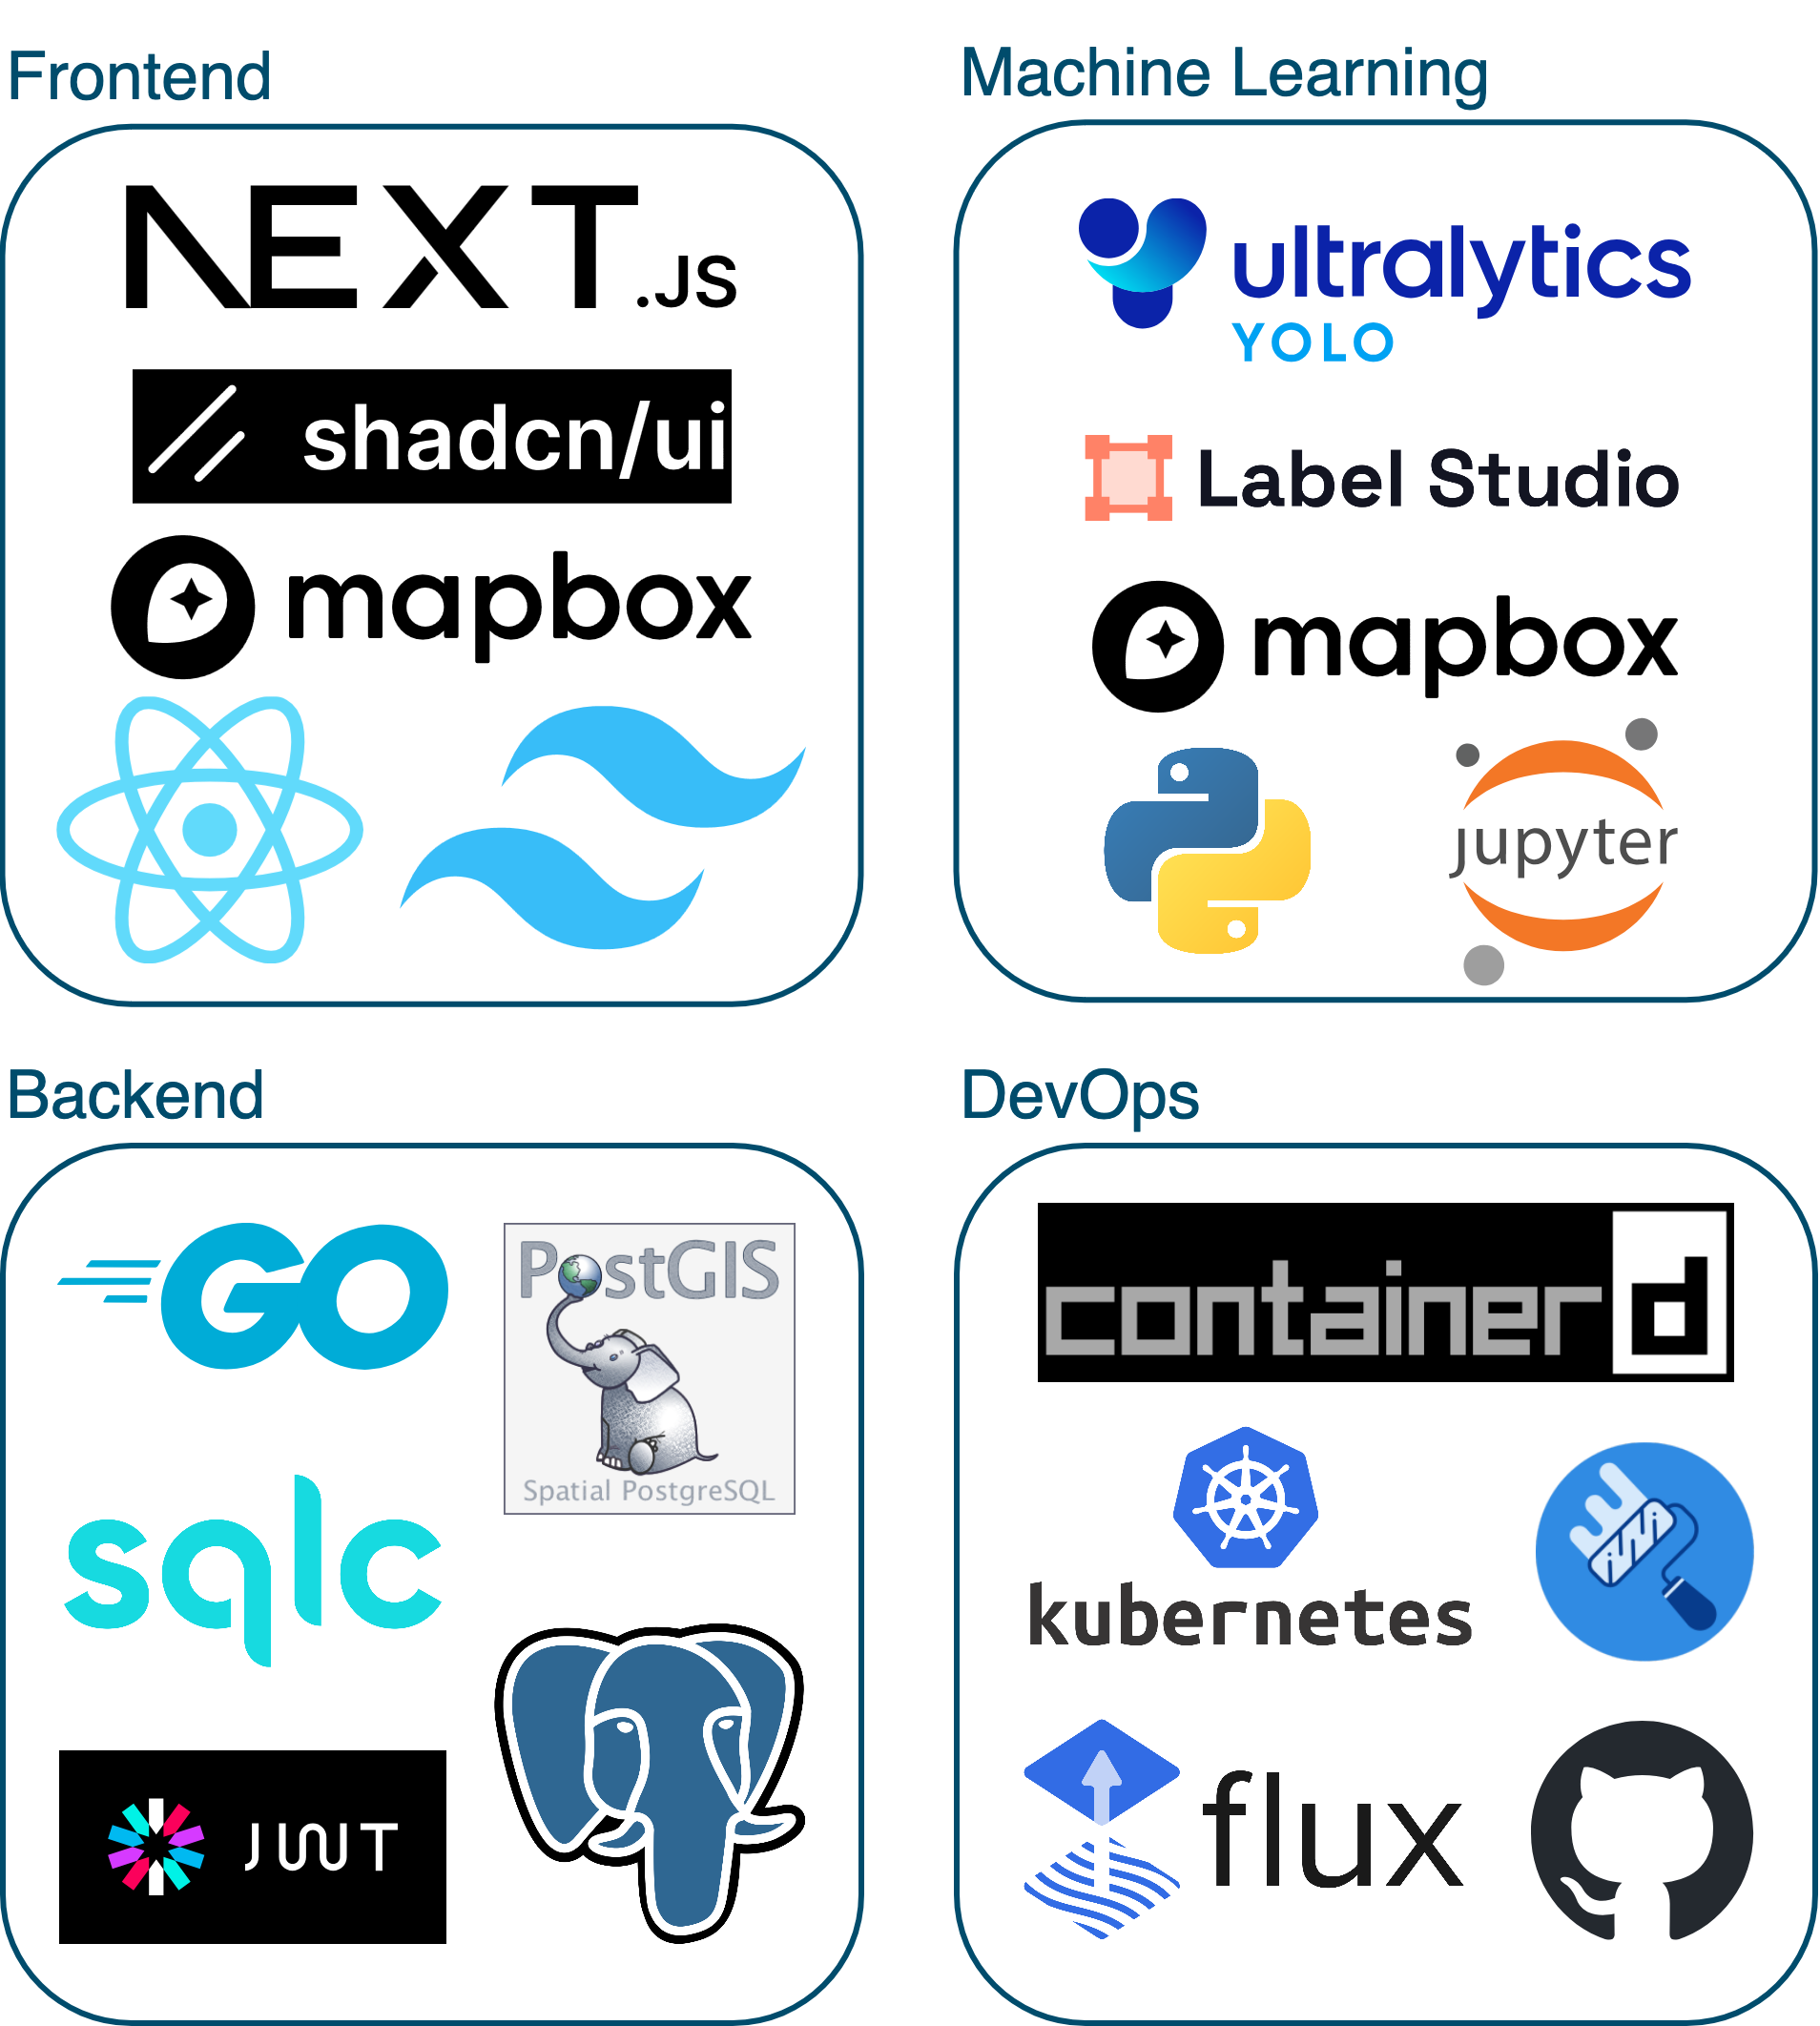
\includegraphics[width=0.8\columnwidth]{images/stack_grid.png}
  \caption{Technologies used in \textit{Magpie}}
  \label{fig:tech_stack}
\end{figure}

\subsection{Frontend}
With \textit{Magpie}, we utilized a modern web development stack, integrating
several technologies to optimize performance, scalability, and maintainability.
Below is a breakdown of the primary technologies and their roles in the project.

\vspace{-3mm}
\begin{enumerate}
    \item{\textbf{React:} React is a popular JavaScript library for building
    user interfaces, we used React in conjunction with Next.js to enable a
    component-driven architecture. This allowed for reusable UI components,
    which increased development efficiency and ensured maintainability.}
    \vspace{1.25mm}

    \item{\textbf{Next.js:} Next.js is a React Framework that offers server-side
    rendering (SSR) and static site generation (SSG), both of which are
    advantageous for optimizing load times and improving SEO. In this project,
    Next.js was used as the core frontend framework, enabling us to build a
    performant web application with powerful routing and SSR capabilities.}
    \vspace{1.25mm}

    \item{\textbf{TailwindCSS:} TailwindCSS, a utility-first CSS framework, was
    implemented for styling the application. It enabled rapid UI development by
    providing low-level utility classes, allowing us to avoid writing custom
    CSS. The addition of tailwind-merge and tailwindcss-animate facilitated more
    complex styling and animations.}
    \vspace{1.25mm}

    % Forcing a page break here to keep the list together
    \pagebreak{}

    \item{\textbf{Mapbox GL and React Map GL:} For map-based features, Mapbox GL
    and React Map GL were utilized. Mapbox GL provided the core functionality
    for interactive maps, while React Map GL integrated this into our React
    components efficiently. Deck.gl was also used for advanced visualization
    layers on top of maps, enabling us to display large data sets smoothly.}
    \vspace{1.25mm}

    \item{\textbf{ShadCN/UI:} For building UI components, we incorporated
    ShadCN, a component library designed on top of Radix Primitives. ShadCN
    brings the flexibility of Radix UI while combining it with a more
    opinionated design system, tailored specifically for projects that require
    custom styling with the power of TailwindCSS. This allowed for highly
    customizable, accessible components, with minimal configuration, speeding up
    the development process while maintaining design consistency. ShadCN’s tight
    integration with Radix Primitives helped ensure accessibility standards were
    met without sacrificing flexibility.}
    \vspace{1.25mm}

\end{enumerate}

\noindent{}The integration of these technologies into the project provided a
solid foundation for building a performant, scalable, and user-friendly web
application. From Next.js for SSR to ShadCN for accessible components, each tool
played a crucial role in achieving the project’s goals while maintaining high
standards of code quality, user experience, and performance.

\subsection{Machine Learning}

This project aims to provide a tool that allows Urban Planners to make informed
decisions using multiple data sources. Early on in the project, we identified
that on-street parking detection would be a key feature of the platform,
realising this would be the most difficult element of the machine learning
pipeline, we decided to tackle this first.

\noindent{}To detect parking spots from satellite images, the following steps
are implemented: image acquisition, mask generation, car detection, and finally
parking spot localisation.

\vspace{-3mm}
\begin{itemize}
  \item{First, satellite images and corresponding road map images are retrieved
  for a specific area contained within a bounding box, defined by its top-left
  and bottom-right coordinates, from the Mapbox API.}
  \vspace{1.25mm}

  \item{Next, a binary mask is generated by identifying road pixels based on
  their colour. The majority of roads are depicted in white, though motorways or
  major roads are marked in orange and yellow, which are detected through
  additional colour masks.}
  \vspace{1.25mm}

  % Forcing a page break here to keep the list together
  \pagebreak{}

  \item{The masks are then combined and refined using morphological operations
  to remove additional noise (street names), simplifying the image to isolate
  the roads from other elements.}
\end{itemize}

% We want to maintain paragraphs on the same page where possible \pagebreak{}

\noindent{}We train a model to recognize all cars based on images from our
dataset. We chose the YOLO (You-Only-Look-Once) model because of its popularity
and great results in the object detection task. We started with version 5 and
upgraded to version 8 for its improved accuracy.

\begin{figure}[h]
  \centering
  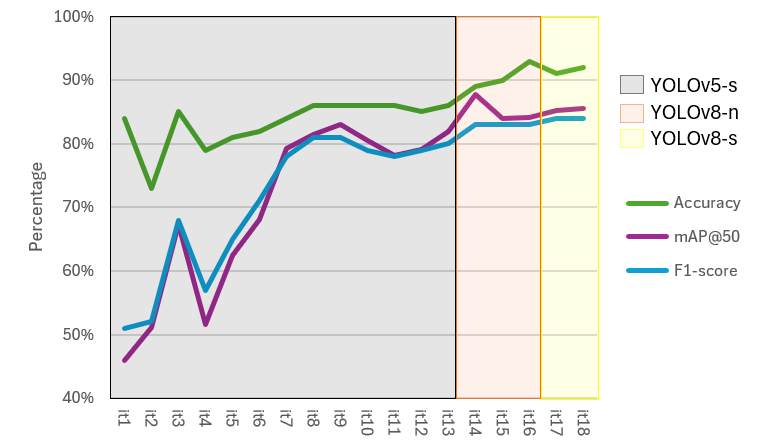
\includegraphics[width=\columnwidth]{images/training_table1.png}
  \caption{Yolo v5 vs Yolo v8 comparison}
  \label{fig:parking_detection}
\end{figure}

\noindent{}Through the training process, accuracy results stagnated caused by
labelling inconsistencies in our dataset. For example, bounding boxes were not
rotated correctly to fit the cars, thus making it harder for the model to
recognize them consistently and with confidence. After cautious re-labelling,
training continued, testing different optimizers, epoch numbers, and patience
thresholds.

\noindent{}This resulted in:
\begin{mdframed}[innerleftmargin=0pt, innerrightmargin=0pt, innertopmargin=0pt, innerbottommargin=0pt]
\begin{align*}
\text{Accuracy:} & \quad 92\% \\
\text{Precision:} & \quad 100\% \\
\text{Confidence Threshold (Precision):} & \quad 75.1\% \\
\text{Recall:} & \quad 98\% \\
\text{F1-Score:} & \quad 84\% \\
\text{mAP@50:} & \quad 85.6\% \\
\text{Optimal Confidence Threshold (F1 curve):} & \quad 35.8\%
\\
\end{align*}
\end{mdframed}

\noindent{}Next, the fine-tuned YOLOv8 model is used to detect cars in the
satellite images. The road mask is overlaid over the output of the initial model
to exclude cars on the road, resulting in a set of cars which are not on the
road, we have decided to consider these parked cars. Once the parked cars are
identified, we then convert the marked cars into coordinates.

\begin{figure}[h]
    \centering
    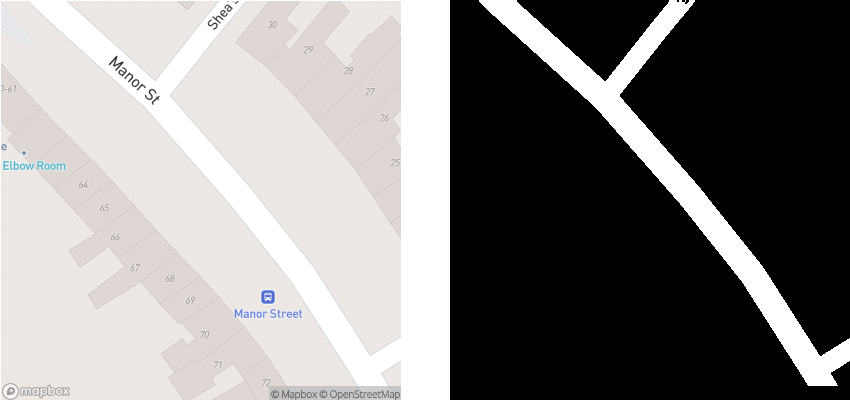
\includegraphics[width=\columnwidth]{images/mask_and_mapbox.png}
    \caption{Example of mask and mapbox image}
    \label{fig:mask_and_mapbox}
\end{figure}

\noindent{}Finally, the locations of all parking spots found within the
specified bounding box are saved in a CSV file and subsequently sent to the
PostgreSQL database.

\begin{figure}[h]
    \centering
    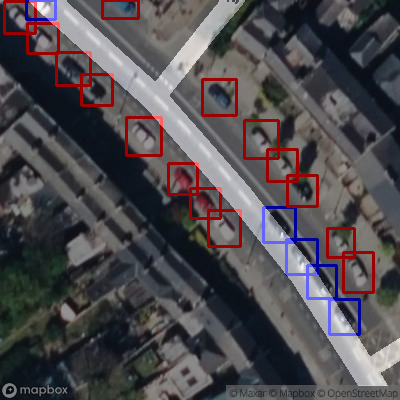
\includegraphics[width=0.65\columnwidth]{images/opacity_mask.png}
    \caption{Parking with mask applied}
    \label{fig:parking_detection}
\end{figure}

\subsection{Backend}

Supplying the data extracted by the machine learning model to the frontend is
the task of two separate backend applications. Both interact with a PostgreSQL
database, which acts as the heart of the system.

\noindent{}\textbf{Why split the backend?}

\noindent{}The backend is split into two components -- a private and a public
backend. This is achieved by utilising build tags to compile two applications
with two feature sets from a shared Golang codebase. Using a split architecture
for the backend provides two key advantages:

\vspace{-3mm}
\begin{itemize}
  \item{\textbf{Scalability:} The decision to deploy the application containers
  using Kubernetes incentivize the use of smaller services. This allows each
  component of the service to be scaled independently. Since each service will
  encounter high traffic situations under different circumstances, this
  flexibility is advantageous.}

  \item{\textbf{Security:} The private backend is strictly accessible from
  inside the cluster itself. This makes the points data essentially immutable to
  the public backend. Even if a malicious actor manages to gain elevated
  privileges on their user account, the public backend is unable to make changes
  to point data.}
\end{itemize}
\vspace{-3mm}

\begin{figure}[h]
  \centering{
  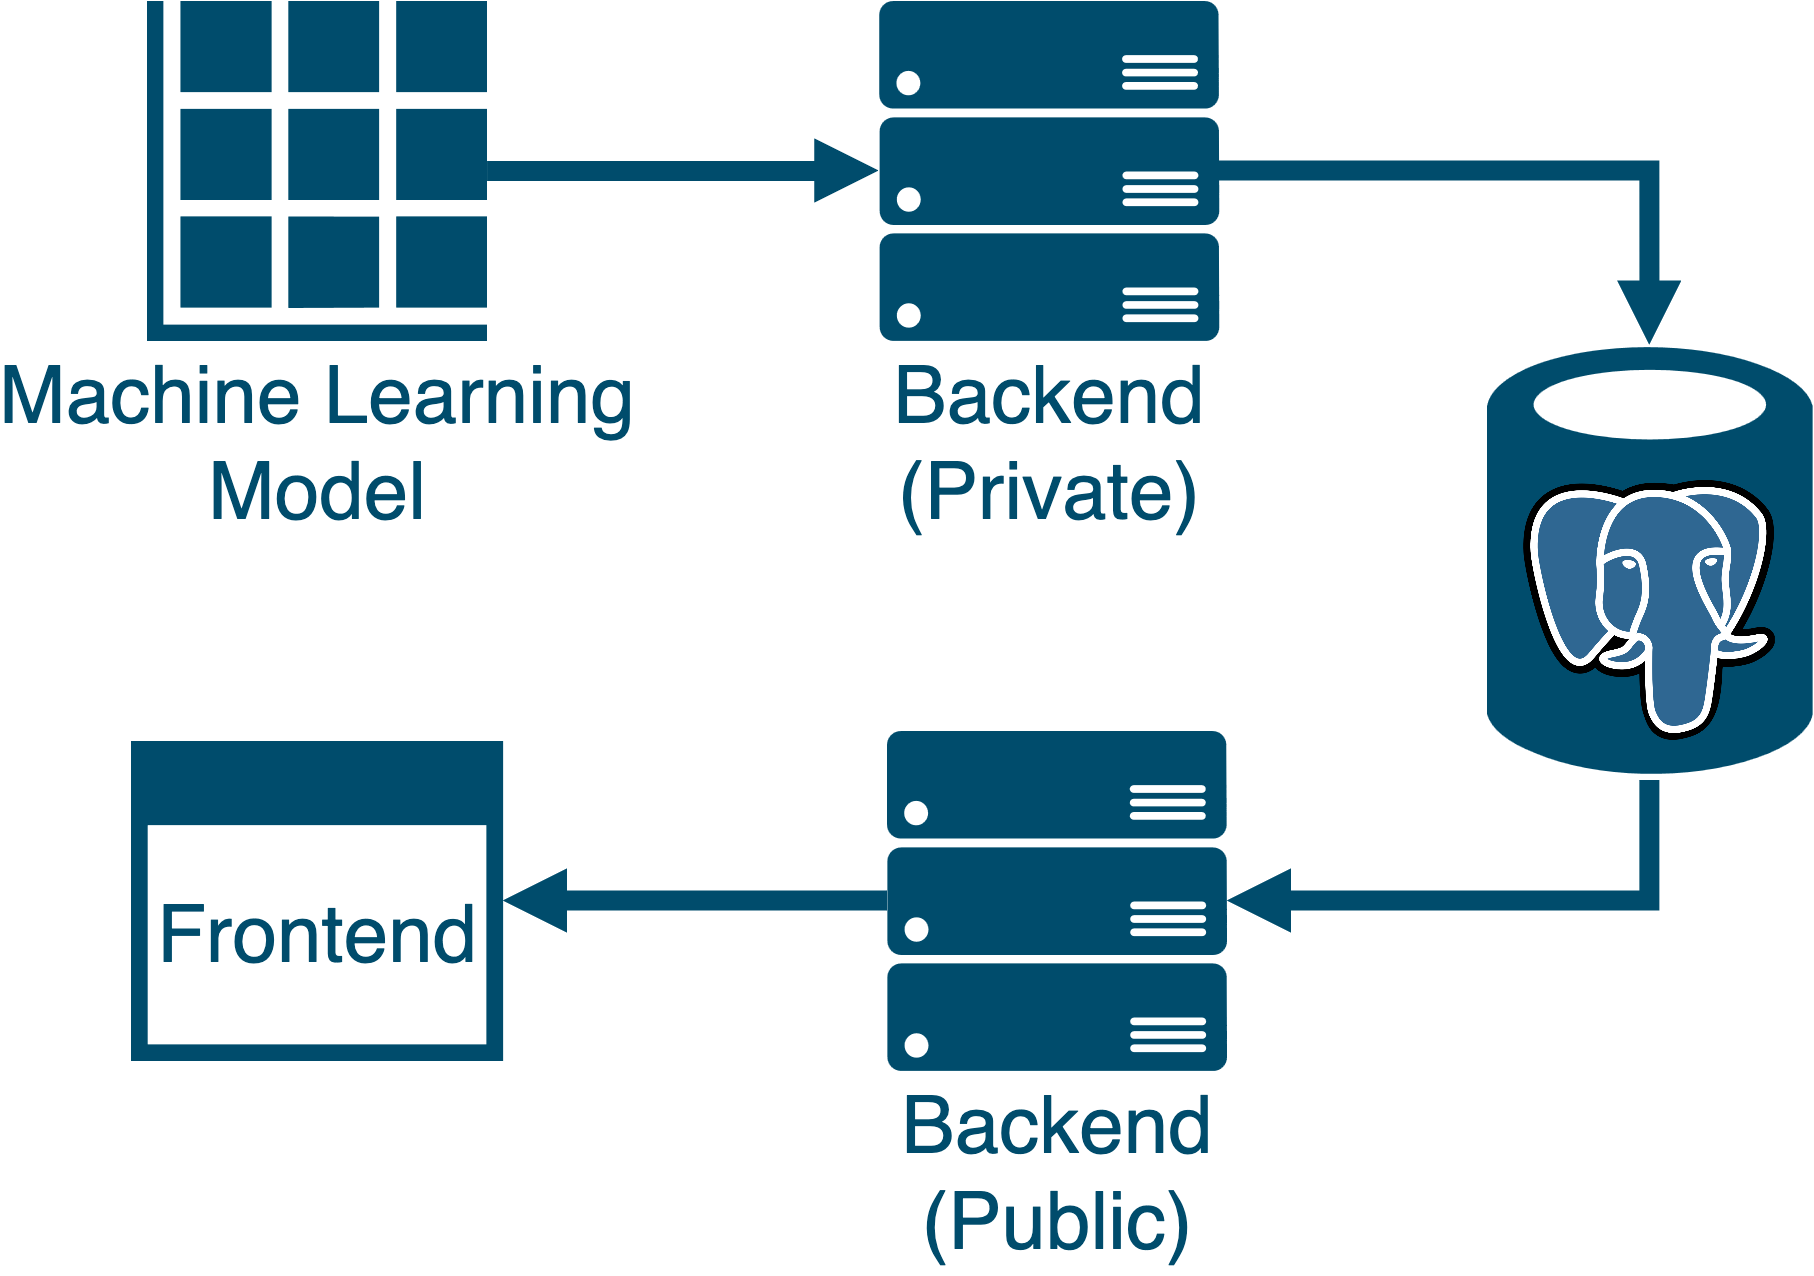
\includegraphics[width=0.80\columnwidth]{images/dataflow_backend2.png}
  \caption{Example of backend data flow}
  \label{fig:dataflow_backend2}
  }
\end{figure}

% Forcing a page break here to keep the list together
\pagebreak{}

\noindent{}\textbf{Private Backend}

\noindent{}The private backend serves as an interface between the machine
learning model and the database. It takes in the extracted datapoints via a REST
API and inserts them into the database. It is accessible strictly from IP
addresses inside the cluster.

\noindent{}\textbf{Public Backend}

\noindent{}The public backend serves as an interface between the frontend and
the database. It exposes routes to manage user accounts (CRUD) and request the
data extracted by the machine learning model (read-only).

\noindent{}The authentication is handled using JSON Web Tokens and bcrypt. Some
routes are protected depending on access level (public, logged-in, user-only).

\subsection{DevOps}

From the beginning, the \textit{Magpie} project was intended to be built as
fast, and with the least amount of friction, as possible. To achieve this, we
implemented as many DevOps strategies as we had the skill and knowledge to
implement.

\noindent{}\textbf{Kubernetes}

\noindent{}The core of our deployment strategy is Kubernetes. Kubernetes is a
container orchestration platform that allows us to deploy, scale, and manage
containerized applications. As mentioned in previous sections, designing an
application for Kubernetes grants us opportunities as well as design
considerations. For example, we can easily configure our application to load
balance- but to allow for this, we need to adopt a microservice architecture.

\noindent{}However, while Kubernetes is a great deployment tool, it can be difficult to
maintain consistency between the state of the cluster and our codebase. To solve
this we use \textit{Flux}. Flux watches a Git repository and (on an interval)
replicates the Kubernetes config to the cluster.

% Forcing a page break here to keep the list together
\pagebreak{}

\noindent{}\textbf{Continuous Integration}

\noindent{}Flux only solves half of the problem. We also need to ensure that our
containerised application is built, otherwise, while Flux will replicate the
config, it will not update the application. To solve this, we use \textit{GitHub
Actions.}. We have implemented several Actions which build the application. Once
built, the containers are pushed to the \textit{GitHub Container Registry}.

\noindent{}There are scenarios where we may have a built container but may not
want to deploy it immediately. As such, we make use of \textit{Mend Renovate}.
Renovate is a tool that automatically updates dependencies in Git repositories
by creating pull requests. Whenever we build a new version of the code, Renovate
will create a pull request to update the container version. This allows us to
keep our deployments up to date, but also allows us to manually chose
\textit{when} to update.